\section{Preliminaries: Problem Formulation}
\label{sec:preliminaries}

We begin by formally defining the vaccine allocation problem on contact networks.
Our formulation consists of two components: (1) individual-level epidemic dynamics
modeled as a continuous-time Markov process (CTMP), and (2) the vaccine allocation
objective formulated as a stochastic optimal control problem.

% ============================================
\subsection{Individual-level Epidemic Dynamics}
\label{sec:ctmp_dynamics}

We model epidemic spread as a CTMP on a contact network $\mathcal{G} = (V, E)$,
where $V = \{1, \ldots, N\}$ represents individuals and $E$ represents potential
transmission pathways.

\subsubsection{Population Heterogeneity}

The population is partitioned into three risk groups based on epidemiological characteristics:
\begin{itemize}
    \item \textbf{Baseline group} ($g=0$): $f_0 = 67.2\%$ of population
    \item \textbf{High-risk group} ($g=1$): $f_1 = 16.8\%$ (elderly, immunocompromised; high mortality)
    \item \textbf{High-contact group} ($g=2$): $f_2 = 15.0\%$ (essential workers, youth; high transmission)
\end{itemize}

The contact network is generated according to a group-structured model with contact matrix
$\mathbf{C} \in \mathbb{R}^{3 \times 3}$:
\begin{equation}
\mathbf{C} = \begin{bmatrix}
0.165 & 0.1 & 0.175 \\
0.1 & 0.0 & 0.002 \\
0.175 & 0.002 & 0.132
\end{bmatrix}
\end{equation}
where $C_{gh}$ governs the edge probability between individuals in groups $g$ and $h$.
This matrix reflects empirical observations~\citep{mistry2021inferring} that high-risk
individuals have limited contact (especially with high-contact groups), while high-contact
individuals exhibit dense intra-group connectivity.

\subsubsection{Disease States and Transitions}

Each individual $i \in V$ occupies one of six mutually exclusive disease states:
\begin{equation}
s_i(t) \in \mathcal{X} := \{\text{S}, \text{E}, \text{I}, \text{R}, \text{V}, \text{D}\}
\end{equation}
representing Susceptible, Exposed (latent), Infected (infectious), Recovered,
Vaccinated, and Dead, respectively. The state transition dynamics are illustrated
in Figure~\ref{fig:state_diagram}.

The key feature distinguishing our model from population-level ODE approaches is the
\textbf{network-dependent force of infection}. For individual $i$ at time $t$:
\begin{equation}
\lambda_i(t) = \beta \cdot \frac{|\{j \in \mathcal{N}(i) : s_j(t) = \text{I}\}|}{|\mathcal{N}(i)|}
\label{eq:foi}
\end{equation}
where $\mathcal{N}(i)$ denotes the set of graph neighbors of $i$, and $\beta$ is the
baseline transmission rate. This formulation captures the fundamental insight that
infection risk depends on \emph{local} network structure rather than global population statistics.

\begin{figure}[t]
\centering
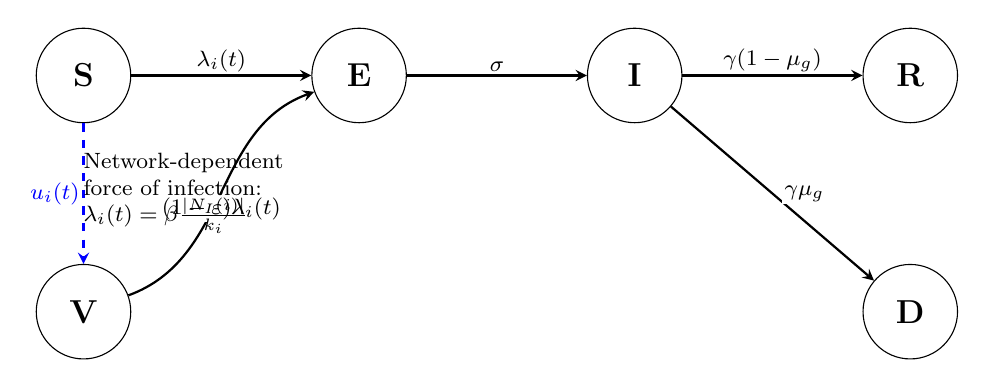
\begin{tikzpicture}[
    state/.style={circle, draw, minimum size=1.2cm, font=\bfseries\large},
    arrow/.style={->, >=stealth, thick},
    control/.style={->, >=stealth, thick, blue, dashed},
    label/.style={font=\footnotesize, midway, fill=white, inner sep=1pt}
]
    % Nodes
    \node[state] (S) at (0,0) {S};
    \node[state] (E) at (3.5,0) {E};
    \node[state] (I) at (7,0) {I};
    \node[state] (R) at (10.5,0) {R};
    \node[state] (V) at (0,-3) {V};
    \node[state] (D) at (10.5,-3) {D};

    % Transitions
    \draw[arrow] (S) -- node[label, above] {$\lambda_i(t)$} (E);
    \draw[arrow] (E) -- node[label, above] {$\sigma$} (I);
    \draw[arrow] (I) -- node[label, above] {$\gamma(1-\mu_g)$} (R);
    \draw[arrow] (I) -- node[label, right, xshift=3pt] {$\gamma\mu_g$} (D);
    \draw[control] (S) -- node[label, left] {$u_i(t)$} (V);
    \draw[arrow] (V) to[out=20, in=200] node[label, below] {$(1-\varepsilon)\lambda_i(t)$} (E);

    % Annotations
    \node[font=\footnotesize, align=left, text width=3.5cm] at (1.75, -1.5)
        {Network-dependent\\force of infection:\\$\lambda_i(t) = \beta \frac{|N_I(i)|}{k_i}$};
\end{tikzpicture}
\caption{CTMP state transition diagram. Solid arrows represent disease progression;
dashed blue arrow indicates vaccination control. Unlike mean-field ODE models,
$\lambda_i(t)$ depends on individual $i$'s local network neighborhood.}
\label{fig:state_diagram}
\end{figure}

State transitions occur stochastically with the following rates (using discrete-time
approximation with $\Delta t = 1$ day):

\paragraph{Infection ($\text{S} \to \text{E}$, $\text{V} \to \text{E}$).}
\begin{align}
P(s_i(t+1) = \text{E} \mid s_i(t) = \text{S}) &= 1 - \exp(-\lambda_i(t)) \approx \lambda_i(t) \\
P(s_i(t+1) = \text{E} \mid s_i(t) = \text{V}) &= (1-\varepsilon)\lambda_i(t)
\end{align}
where $\varepsilon = 0.8$ is the vaccine efficacy.

\paragraph{Disease progression ($\text{E} \to \text{I}$).}
\begin{equation}
P(s_i(t+1) = \text{I} \mid s_i(t) = \text{E}) = \sigma = \frac{1}{4}
\end{equation}
corresponding to a mean latent period of 4 days.

\paragraph{Recovery or death ($\text{I} \to \{\text{R}, \text{D}\}$).}
\begin{equation}
P(s_i(t+1) \in \{\text{R}, \text{D}\} \mid s_i(t) = \text{I}) = \gamma = \frac{1}{7}
\end{equation}
with conditional probabilities $P(\text{D} \mid \text{outcome}) = \mu_{g(i)}$ and
$P(\text{R} \mid \text{outcome}) = 1 - \mu_{g(i)}$, where the group-specific
death rates are $\mu_0 = \mu_2 = 0.01$ and $\mu_1 = 0.1$ (10-fold higher for high-risk).

\paragraph{Vaccination ($\text{S} \to \text{V}$).}
This is the \emph{control action}: $P(s_i(t+1) = \text{V} \mid s_i(t) = \text{S}) = u_i(t)$,
where $u_i(t) \in [0,1]$ is the vaccination probability determined by the policy.

The complete CTMP simulation algorithm is provided in Algorithm~\ref{alg:ctmp}.

\begin{algorithm}[t]
\caption{CTMP Simulation (one time step)}
\label{alg:ctmp}
\begin{algorithmic}[1]
\STATE \textbf{Input:} States $\{s_i(t)\}_{i=1}^N$, graph $\mathcal{G}$, actions $\{u_i(t)\}$
\STATE \textbf{Output:} Next states $\{s_i(t+1)\}_{i=1}^N$
\FOR{each individual $i \in V$}
    \IF{$s_i(t) = \text{S}$ and $\text{Bernoulli}(u_i(t))$}
        \STATE $s_i(t+1) \gets \text{V}$
    \ELSIF{$s_i(t) \in \{\text{S}, \text{V}\}$}
        \STATE $\lambda_i \gets \beta \cdot |\{j \in \mathcal{N}(i) : s_j(t) = \text{I}\}| / |\mathcal{N}(i)|$
        \STATE $\lambda_i \gets (1-\varepsilon)\lambda_i$ if $s_i(t) = \text{V}$
        \IF{$\text{Bernoulli}(\lambda_i)$}
            \STATE $s_i(t+1) \gets \text{E}$
        \ENDIF
    \ELSIF{$s_i(t) = \text{E}$ and $\text{Bernoulli}(\sigma)$}
        \STATE $s_i(t+1) \gets \text{I}$
    \ELSIF{$s_i(t) = \text{I}$ and $\text{Bernoulli}(\gamma)$}
        \STATE $s_i(t+1) \gets \text{D}$ if $\text{Bernoulli}(\mu_{g(i)})$ else $\text{R}$
    \ENDIF
\ENDFOR
\end{algorithmic}
\end{algorithm}

% ============================================
\subsection{Vaccine Allocation as Stochastic Optimal Control}
\label{sec:oc_formulation}

The vaccine allocation problem can be theoretically formulated as a finite-horizon
stochastic optimal control problem. Let $s_t = (s_1(t), \ldots, s_N(t))$ denote the
system state and $u_t = (u_1(t), \ldots, u_N(t))$ the control vector. The objective is:

\begin{equation}
\begin{aligned}
\min_{u_0, \ldots, u_{T-1}} \quad & J(u) = \mathbb{E}\left[ \sum_{t=0}^{T-1} L(s_t) \right] \\
\text{subject to} \quad & s_{t+1} \sim P(\cdot \mid s_t, u_t) \quad \text{(CTMP dynamics)} \\
& \sum_{i=1}^N u_i(t) \cdot \mathbb{I}[s_i(t) = \text{S}] \leq V_{\max} \quad \forall t \\
& u_i(t) \in [0, 1] \quad \forall i, t
\end{aligned}
\label{eq:oc_problem}
\end{equation}

where the stage cost $L(s_t) = |\{i : s_i(t) = \text{I}\}| + 10 \cdot |\{i : s_i(t) = \text{D}\}|$
penalizes infections and deaths (with deaths weighted 10× higher), and $V_{\max}$ is the
daily vaccine supply constraint.

This formulation has the structure of a \textbf{stochastic optimal control problem} on a
high-dimensional, network-coupled Markov process. In the continuous-time limit, it
corresponds to minimizing:
\begin{equation}
J(u) = \mathbb{E}\left[ \int_0^T L(s(t)) \, dt \right]
\end{equation}
subject to the stochastic differential equation governing the CTMP.

\paragraph{Comparison to population-level optimal control.}
Recent work~\citep{师兄论文} has successfully applied optimal control theory to
vaccine allocation at the \emph{population level}, where the state is a 30-dimensional
vector representing disease compartment densities for 3 groups. That formulation is
computationally tractable (solvable in seconds via direct collocation methods) because:
(1) the state/control dimensionality is low, (2) the dynamics are deterministic ODEs,
and (3) the problem exhibits separability across groups.

% ============================================
\subsection{Computational Intractability of Direct Optimal Control}
\label{sec:intractability}

Despite the elegant theoretical formulation~\eqref{eq:oc_problem}, \textbf{direct
optimal control methods are computationally intractable} for our individual-level
problem due to the following challenges:

\subsubsection{Curse of Dimensionality}

The state space has cardinality $|\mathcal{X}|^N = 6^{2000} \approx 10^{1554}$, vastly
exceeding the size of any problem solvable by dynamic programming or value iteration.
Even continuous-state approximations yield a $12{,}000$-dimensional state vector
(6 states $\times$ 2000 individuals), compared to the 30-dimensional ODE system.
Similarly, the control space is $[0,1]^{2000}$—three orders of magnitude larger than
population-level formulations.

\subsubsection{Stochastic Dynamics}

Solving stochastic optimal control problems requires computing expectations over
all possible realizations of random events. In our CTMP, each time step involves
$N$ independent Bernoulli trials (for infections, disease progression, deaths).
Computing $\mathbb{E}[\cdot]$ exactly would require summing over $2^N$ outcomes per
time step—an exponentially intractable operation. Continuous-time stochastic control
techniques (e.g., solving the Hamilton-Jacobi-Bellman PDE) are similarly infeasible
in dimension $10^4$.

\subsubsection{Network Coupling}

Standard optimal control theory assumes separable dynamics: $\dot{s}_i = f_i(s_i, u_i)$.
Our CTMP violates this due to network-dependent infection~\eqref{eq:foi}: the transition
probability for individual $i$ depends on the states of all neighbors $\mathcal{N}(i)$.
This coupling, mediated by the graph structure $\mathcal{G}$, introduces nonlocal
interactions that break the standard factorization assumptions underlying scalable
control algorithms.

\paragraph{Consequence: Reinforcement Learning as Approximation.}
Given these fundamental computational barriers, we turn to \textbf{reinforcement learning}
as an approximate solution method. RL sidesteps the intractability by:
(1) using function approximation (neural networks) to represent policies in high dimensions,
(2) estimating expectations via Monte Carlo sampling rather than exact computation,
and (3) learning policies directly from simulated experience without solving the
Bellman equation globally. However, RL suffers from poor sample efficiency, which
motivates our use of prior knowledge from tractable ODE-level optimal control
solutions (Section~\ref{sec:our_approach}).

\vspace{1em}
\noindent\textbf{Remark.}
The intractability analysis above establishes a clear dichotomy: population-level
vaccine allocation (师兄论文) is amenable to classical optimal control, while
individual-level allocation on networks requires approximate methods. Our contribution
lies in bridging these regimes by using ODE-based optimal control to guide RL-based
individual-level optimization.

% ============================================
% ============================================

\section{Our Approach: Prior-Guided Reinforcement Learning with Diffusion}
\label{sec:our_approach}

Having established that direct optimal control is intractable for individual-level
CTMP (Section~\ref{sec:intractability}), we now present our solution: a three-stage
framework that combines macro-level optimal control, diffusion models, and reinforcement
learning. The key idea is to leverage \emph{tractable} population-level optimal control
solutions as priors to accelerate \emph{intractable} individual-level RL.

\subsection{Overview}

Our approach consists of three stages (Figure~\ref{fig:pipeline}):

\begin{enumerate}
    \item \textbf{Macro-level expert generation (M1):} Solve group-level optimal control
    problems on ODE dynamics using existing methods~\citep{师兄论文}, producing expert
    trajectories $\{\tau_{\text{ODE}}^{(k)}\}$.

    \item \textbf{Diffusion prior learning (M2):} Lift macro-level actions to individual-level
    via a degree-risk weighted algorithm, then train a conditional diffusion model
    $p_\theta(a \mid s)$ on the lifted data to capture expert strategy distributions.

    \item \textbf{Prior-guided reinforcement learning (M3):} Train a PPO agent on the
    individual-level CTMP environment, regularized by KL divergence to the diffusion prior:
    \begin{equation}
    \mathcal{L} = \mathcal{L}_{\text{PPO}} + \beta \cdot D_{\text{KL}}(\pi_\phi \| p_\theta)
    \end{equation}
    where $\beta$ decays over training to gradually shift from imitation to optimization.
\end{enumerate}

\textit{[Sections 4.1-4.4 to be written with detailed algorithms and architectures]}

\subsection{Macro-level ODE Expert Generation}
\label{sec:ode_expert}

\textit{[To be written]}

\subsection{Macro-to-Micro Lifting Algorithm}
\label{sec:lifting}

\textit{[To be written]}

\subsection{Conditional Diffusion Model for Strategy Prior}
\label{sec:diffusion}

\textit{[To be written]}

\subsection{Prior-Guided Reinforcement Learning}
\label{sec:rl}

\textit{[To be written]}
